\section{pyWATTS}
\label{sec:pywatts}

In order to combine the models in a joint environment 
and reuse steps like the calculation of the pinball loss, 
it makes sense to use some kind of pipeline structure for the code. 
\Textcite{Heidrich2021} introduced 
pyWATTS\footnote{\url{https://github.com/KIT-IAI/pyWATTS}}, a framework 
for creating pipelines for time series forecasting. 

\begin{figure}[h]%
    \centering
    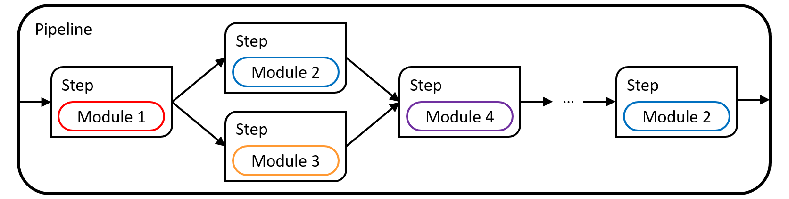
\includegraphics[width=0.9\textwidth]{plots/pywatts-schematic.pdf}
    \caption[pywATTS schematic]{pyWATTS schematic from \Textcite{Heidrich2021}. 
    Each step of the algorithm can be added in a single pipeline module. 
    A module can be used multiple times like for training and forecasting purposes.}
    \label{fig:pywatts-schematic}%
\end{figure}

pyWATTS can create different stages for each subtask of a pipeline like 
data pre- and postprocessing, model training, model testing and 
rendering predictions into images, a schematic of the pipeline 
can be found in Figure \ref{fig:pywatts-schematic}. Wrappers for scikit-learn 
modules are already implemented so the creation of a pipeline 
for scikit-learn models is relatively straightforward. 
For other neural network models, one can simply create a class that inherit the 
\texttt{BaseWrapper} class. The \texttt{fit}- and \texttt{transform}-methods 
need to be implemented to train the model and make predictions with it. 
Simple transformations like for example the NNQF preprocessing step can be 
wrapped by a \texttt{FunctionModule} and inserted into the pipeline.
For each stage in the pipeline, one can output the data of the model 
with callbacks like the \texttt{CSVCallback} to save \texttt{csv}-files or 
the \texttt{ImagePlotCallback} to save images.